\documentclass[12pt,a4paper,notitlepage]{report}
\usepackage[utf8]{inputenc}
\usepackage[czech,english]{babel}
\usepackage[pdftex]{graphicx} %pro vkládání obrázků v eps
\usepackage{hyperref} %pro kliknutelné linky
%\usepackage{sectsty} % pro jednoduché přestylování nadpisů
\usepackage[round]{natbib} %pro bibliografii a citace
\usepackage{tabularx} %pro lepsi tabulky (hlavne v sekci symboly)
\usepackage{booktabs} %pro hezke tabulky v dokumentu
\usepackage[small,bf,belowskip=0.2cm]{caption} %změna stylu popisku a mezery před a za
\usepackage{siunitx} %pro sazbu fyzikálních jednotek
\usepackage[top=2.5cm, bottom=2.5cm, left=2.5cm, right=2cm]{geometry} %nastaveni okraju a vzdalenosti cislovani
\usepackage{subfig} %subfloat je nejaky divny, takze navrat k subfig-u


%vypne vypisovani Kapitola u \chapter
\makeatletter
\def\@makechapterhead#1{%
  \vspace*{\p@}%
  {\parindent \z@ \raggedright \normalfont
    \interlinepenalty\@M
     \fontsize{21pt}{1.5}\selectfont \bfseries \thechapter\ \hspace{10pt} #1\par\nobreak
    \vskip 22\p@
  }}
\makeatother{}

%aby stejne vypadala i chapter*
\makeatletter
\def\@makeschapterhead#1{%
  \vspace*{\p@}%
  {\parindent \z@ \raggedright \normalfont
    \interlinepenalty\@M
     \fontsize{21pt}{1.5}\selectfont \bfseries #1\par\nobreak
    \vskip 22\p@
  }}
\makeatother{}

%nastaveni zobrazovani cisel jak je u nas zvykem :)
\sisetup{output-decimal-marker={,},exponent-product = \cdot, list-final-separator = { a }  }

%nove prikazy
\newcommand{\keps}{$k\mbox{-}\epsilon$}
\newcommand{\volproc}[1]{\num{#1}\,obj.\,\%}


%\sectionfont{\fontsize{14pt}{1.5}\selectfont}
%\subsectionfont{\fontsize{12pt}{1.5}\selectfont}

\addtocontents{toc}{\protect\thispagestyle{empty}} %odstraní číslování na stránce obsahu

\begin{document}
	\pagestyle{empty} 
	\selectlanguage{czech}
	\begin{center}
{\Large VYSOKÁ ŠKOLA CHEMICKO-TECHNOLOGICKÁ V PRAZE\\}
{\large Fakulta chemicko-inženýrská\\
\textbf{Ústav chemického inženýrství}\\}
\vspace{15mm}

\begin{figure}[!h]
\begin{center}
\includegraphics[angle=0,width=27mm]{images/logo_vscht.eps}
\end{center}
\end{figure}

\vspace{25mm}

{\huge \textbf{CFD simulace\\}}
\vspace{10mm}
{\Large \textbf{SVK 2011\\}}
\end{center}
\vspace{35mm}

%\null
%\vfill

\begin{tabular}{p{50mm}lp{50mm}}
Vypracoval: & \textbf{Bc.\,Tomáš Antecký}\\
\\
Vedoucí práce: & Doc.\,Dr.\,Ing.\,Milan Jahoda \\

\\
Studijní program: & Procesní inženýrství a informatika \\
\\
Studijní obor: & Chemické inženýrství, bioinženýrství \\
	& a matematické modelování procesů\\
\end{tabular}

	\section*{Souhrn}
Následující práce se zabývá simulací procesu suspendace v mechanicky míchané nádobě pomocí metody počítačové dynamiky tekutin. Hlavním cílem bylo stanovit výšku suspezního mraku a posoudit vliv modelu pro koeficient odporu na distribuci pevné fáze. Zkoumaný systém se skládal z válcové nádobou s plochým dnem o vnitřním průměru $T=\SI{0.29}{\meter}$. Pevnou fázi tvořily kuličky z PVC o koncentraci 5, 10 a \volproc{15} a jako kapalná vsádka byla použita voda a polyvinylpyrrolidon. Výška plnění byla zvolena $H=T$ a k promíchání bylo použito šestilopatkové míchadlo se šikmo skloněnými lopatkami (úhel zkosení \SI{45}{\degree}). K vlastní simulaci byl využit komerční software \flu{} 12.1.4 do kterého bylo implementováno několik modelů pro koeficient odporu v podobě uživatelem definovaných funkcí. Pro popis vícefázového proudění byly použity přístupy Eulerian-Eulerian a Eulerian-Granular spolu se standardním \keps{} turbulentním modelem. Výsledky získané numerickou simulací dobře korespondovaly s experimentálním měřením. Zvláště dobré shody bylo především dosaženo v případech, kdy objemový zlomek pevné fáze činil \proc{5} a \proc{10}.

	\selectlanguage{english}
	\section*{Summary}
The following thesis is dealing with simulation of suspension in a mechanically stirred tank by using computational fluid dynamics. The main goal was to determine the height of suspension cloud and asses the impact of the model for the drag coefficient on the distribution of solid phase. The studied system consisted of a flat bottom cylindrical tank with an inner diameter $T=\SI{0.29}{\meter}$. The solid phase was formed of PVC particles and its concentration was 5, 10 and \volfrac{15}. Tap water and polyvinylpyrrolidone were used as working liquid. The height of filling was chosen to $H=T$ and agitation was provided by pitched six-blade turbine (the pitch angle \SI{45}{\degree}). The simulations were done by commercial software \flu{} 12.1.4, which contained several drag coefficient models implemented in the form of user-defined functions. Eulerian-Eulerian and Eulerian-Granular approaches together with standard \keps{} turbulence modele were used for a description of the multiphase flow. The obtained results corresponded well with experimental measurements. Especially good agreement was found for the simulations when the volume fraction of the solid phase was equal to \proc{5} or \proc{10}.

	\selectlanguage{czech}
	The thesis was worked out at the Department of Chemical Engineering of the Institute of Chemical Technology, Prague from January 2010 to May 2010.

\vspace{16cm}
"I hereby declare that I have developed this thesis independently while noting all resources used, as well as all co-authors. I consent to the publication of this thesis under Act No. 111/1998, Coll., on universities, as amended by subsequent regulations. I have been informed of all duties and obligations applicable under Act No. 121/2000, Coll., the Copyright Act, as amended by subsequent regulations."

\vspace{1cm}
\noindent
Prague, May 10, 2010\\

\hspace{10cm}
Tomáš Antecký
	\section*{Poděkování}
Thanks goes to all l33t hax0rz.
	\tableofcontents
	\pagestyle{plain}
    \setlength{\baselineskip}{1.5\baselineskip}
	\setcounter{page}{0}
	\chapter{Teoretická část}
\section{Suspendace}
Smyslem suspendace v~mechanicky míchaných nádobách je udržení pevných částic ve vznosu tak, aby došlo ke zintenzivnění transportu hmoty a tepla mezi kapalinou a pevnou fází. Pro dosažení tohoto stavu je třeba systému dodat energii v~podobě mechanické práce. K~vykonání této práce se používají rozmanité typy mechanických míchadel, které jsou voleny podle konkretního charakteru dané úlohy. Dodaná energie poté vede k~vytvoření turbulentního proudění, jenž uvede částice pevné fáze do vznosu a následně je rozptýlí v~kapalině. Nutnou podmínkou pro zajištění tohoto vznosu je potřeba, aby výsledná vertikální složka síly působící na částici byla větší než tíhová síla zmenšená o~sílu vztlakovou. Menší částice jejichž hustota je přibližně rovna hustotě kapalina se po dosažení suspenzních podmínek pohybují společně s~kapalinou. Při nižších koncentracích pevné fáze se toto proudění chová spíše jako jednofázový tok. Naopak rychlost pohybu těžších částic se liší od rychlosti kapalné fáze, jenž musí na pevnou fázi působit větší silou k~zabránění jejímu usazování. Výslednou kvalitu vzniklé suspenze ovlivňuje řada faktorů, kde mezi nejvýznamnější patří fyzikální vlastnosti, jak kapalné, tak pevné fáze, provozní podmínky a geometrie systému a míchadla.

\subsection{Stupně suspendace}
Nároky na homogenitu vsádky se liší dle konkretních provozních požadavků. Jedním z~pojmů, který se používá k~popisu míry homogenizace vsádky v~mechanicky míchaných nádobách je stupeň suspendace. Obecně se rozlišují tři stupně suspendace: částečná, úplná a homogenní (obr. \ref{fig:typsus}). 
  
\begin{figure}[h!]
  \centering
  \subfloat[Částečná]{\label{fig:typ1}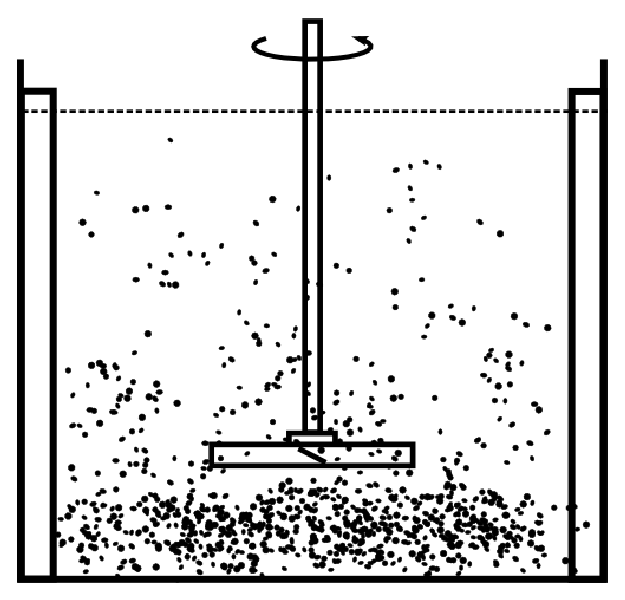
\includegraphics[scale=0.35]{images/typy_suspenzi-1.eps}}
  \qquad
  \subfloat[Úplná]{\label{fig:typ2}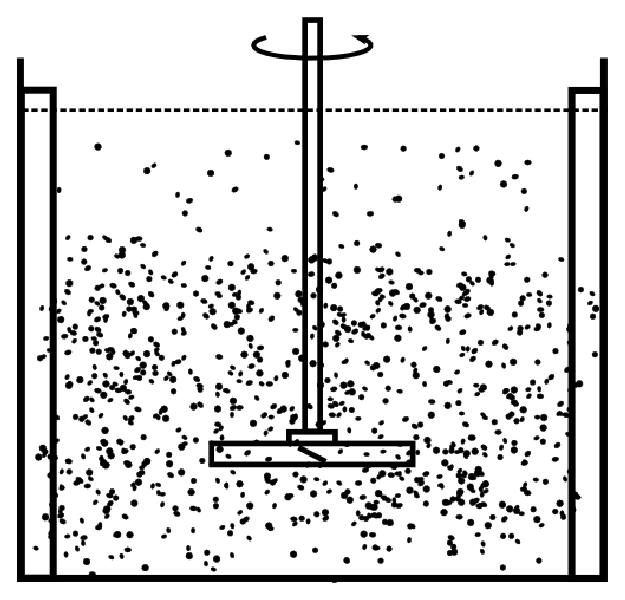
\includegraphics[scale=0.35]{images/typy_suspenzi-2.eps}}
  \qquad
  \subfloat[Homogenní]{\label{fig:typ3}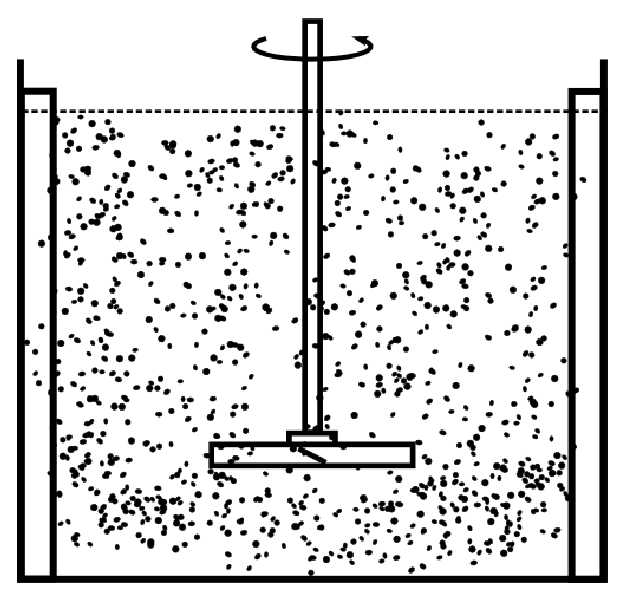
\includegraphics[scale=0.35]{images/typy_suspenzi-3.eps}}
  \caption{Stupně suspendace}
  \label{fig:typsus}
\end{figure}

Při částečné suspendaci lze vizuálně pozorovat pohyb částic pevné fáze pouze v~blízkosti dna nádoby. Toto shlukování má za následek zhoršení přestupu tepla a hmoty, což v~důsledku může snížit rychlost probíhajících chemických reakcí. Z~výše uvedeného vyplývá, že podmínky částečné suspendace jsou postačují pouze při míchaní vysoce rozpustných látek.

Stav úplné suspendace je charakterizován pohybem pevné fáze v~celé nádobě, přičemž žádná částice nezůstává na dně déle než jednu až dvě sekundy. Tato podmínka se někdy označuje jako Zwieteringovo kritérium podle autora, který jako první na základě experimentů navrhl vztah k~výpočtu kritické (minimální) frekvence otáčení míchadla potřebné k~dosažení stavu úplné suspendace. Při tomto stavu je maximální povrch částic vystaven kapalině, což má za následek intenzivní transport hmoty a tepla mezi jednotlivými fázemi.

Posledním stádiem je dosažení stavu homogenní suspendace, při němž částice pevné fáze dosahují prakticky rovnoměrného rozložení v~celém promíchávaném systému. Jakékoliv další zvýšení frekvence míchadla nebo jeho příkonu nemá již prakticky žádný vliv na distribuci pevné fáze. Dosažení stavu homogenní suspendace je často důležité u~procesů, které vyžadují rovnoměrné rozložení částic v~systému. Příkladem takovéhoto procesu může být krystalizace, kde nerovnoměrná koncentrace pevné fáze způsobuje tvorbu míst s~lokálním přesycením, jenž následně negativně ovlivňují kvalitu vzniklých krystalů. Nicméně ve většině případů je postačující dosažení stavu úplné suspendace, který vyžaduje menší množství vykonané práce.

\subsection{Kritická frekvence otáčení míchadla}
Jak již bylo zmíněno v~předcházející kapitole, kritická frekvence otáčení je minimální rychlost otáčení míchadla potřeba k~udržení částic pevné fáze ve vznosu. První kdo navrhl empirickou korelaci k~jejímu výpočtu byl \citet{zwi58}. Jím navržený vztah má tvar:

\begin{equation}
	N_{js} = \left[\frac{g(\rho_{s}-\rho_{l})}{\rho_{l}}\right]^{\num{0.45}}W^{\num{0.13}}d_{p}^{\num{0.2}}D^{\num{-0.85}}\nu^{\num{0.1}}S
	\label{eq:nkrit}
\end{equation} 

\noindent kde $g$ je gravitační zrychlení, $\rho_{s}$ hustota pevné fáze, $\rho_{l}$ hustota kapalné fáze, $W$ relativní hmotnostní zlomek pevné fáze, $d_{p}$ průměr částice pevné fáze, $\nu$ kinematická viskozita a $S$ je bezrozměrná Zwieteringova konstanta, která zohledňuje geometrii systému a míchadla (tab. \ref{tab:S}). Ze vztahu je dobře patrné, že rozdíl hustot jednotlivých fází nejvýznamněji ovlivňuje výslednou kritickou frekvenci otáčení míchadla. Později provedené studie \citep{nie68,bal78,chou97} obecně potvrdily platnost Zwieteringova vztahu. Nicméně \citet{chou97} experimentálně ukázal, že při koncentraci pevné fáze menší než \volproc{2} nebo větší než \volproc{15} se již tato korelace jeví jako nepříliš spolehlivá.

\begin{table}[h!]
\begin{center}
\caption{Zwieteringovy konstanty pro \SI{45}{\degree} PBT}
\label{tab:S}
\begin{tabular}{llr}
\toprule
Šířka lopatky & Světlá výška & Hodnota \\
\midrule

$D/\num{3.5}$ \\
& $T/4$ & \num{4.8} \\
& $T/6$ & \num{4.6} \\
& $T/8$ & \num{3.2} \\
$D/4$ \\
& $T/4$ & \num{4.4} \\
& $T/6$ & \num{4.1} \\
& $T/8$ & \num{3.7} \\

\bottomrule
\end{tabular}
\end{center}
\end{table}

\subsection{Kvalita suspenze (stupeň homogenizace)}
Další užitečnou charakteristikou systému kapalina-pevná fáze je takzvaná kvalita suspenze, což je směrodatná odchylka koncentrace pevné fáze.Často se však dává přednost vyjádření pomocí objemového zlomku pevné fáze. Pro konečný počet $n$ měření lze kvalitu suspenze definovat jako:

\begin{equation}
	\sigma = \sqrt{\frac{1}{n}\sum_{n}^{i=1}\left(\frac{c_{i}}{\bar{c}} - 1\right)^{2}}
	\label{eq:kvasus}
\end{equation}  

\noindent Díky své diskrétní povaze je tato veličina navíc dobře stanovitelná pomocí simulace technikou CFD.

\begin{table}[h!]
\begin{center}
\caption{Zwieteringovy konstanty pro \SI{45}{\degree} PBT}
\label{tab:jj}
\begin{tabular}{cc}
\toprule
Stupeň suspendace & Kvalita suspenze $(\sigma)$ \\
\midrule

Částečná & \num{4.8} \\
Úplná & \num{4.6} \\
Úplná & \num{4.6} \\

\bottomrule
\end{tabular}
\end{center}
\end{table}


\newpage 
\section{Počítačová dynamika tekutin (CFD)}




	\chapter{Literature review}
The suspension of solids has been investigated very extensively over the years. Pioneering was made by \citet{zwi58}, who provided an empirical dimensionless correlation for the  stirred speed at which solids are just suspended. For this velocity is characteristic that no particle remains stationary on the bottom of a tank for more than one or two seconds. Also other authors have experimentally studied the mechanism of suspension of solids in agitated vessels \citep{nie68,bal78,arm98}.   

In the last two decades many researchers have turned their attention to computational fluid dynamics in order to gain better understanding of the phenomena that govern the multiphase systems. Since then CFD has been increasingly employed as an essential tool to minutely analyze the entire flow field and the solid particle distribution. The early CFD simulations   

\section{Particle drag coefficient}


  \chapter*{Seznam symbolů}
\addcontentsline{toc}{chapter}{Seznam symbolů}

\renewcommand\arraystretch{1.5}
\begin{tabularx}{\textwidth}{@{}p{1.0cm} X r@{}}
	$b$ & šířka narážky & \si{\meter} \\
	$c$ & koncentrace & \si{\mole\per\cubic\meter} \\
	$c^{*}$ & bezrozměrná koncentrace & --\\
	$C$ & vzdálenost míchadla ode dna nádoby & \si{\meter} \\
	$C_{D0}$ & odporový koeficient podle Schillera-Naumanna & -- \\ 
	$C_{D}$ & odporový koeficient &  -- \\
	$d_{s}$ & průměr částice & \si{\meter} \\
	$D$ & průměr míchadla & \si{\meter} \\
	
	$\vec{f}_{ext}$ & objemová síla působící na objemový element & \si{\newton\per\cubic\meter} \\
	$\vec{f}_{int}$ & povrchová síla působící na objemový element & \si{\newton\per\cubic\meter} \\
	$\vec{F}_{ad}$ & další síly & \si{\newton} \\
	$\vec{F}_{D}$ & odporová síla & \si{\newton} \\
	$\vec{F}_{g}$ & gravitační síla & \si{\newton} \\
	$\vec{F}_{vz}$ & vztlaková síla & \si{\newton} \\
	$\vec{g}$ & gravitační zrychlení & \si{\meter\per\second\squared} \\
	$H$ & výška plnění nádoby & \si{\meter} \\
	$K$ & koeficient mezifázového sdílení hybnosti & \si{\kilogram\per\cubic\meter\per\second} \\
	$m_{p}$ & hmotnost částice & \si{\kilogram} \\
	
	$p$ & tlak & \si{\pascal} \\
	$\vec{R}$ & mezifázová odporová síla působící na objemový element & \si{\newton\per\cubic\meter} \\
	$Re_{p}$ & Reynoldsovo kritérium pro pevnou částici &  --\\
	$t$ & čas & \si{\second} \\
	$T$ & vnitřní průměr nádoby & \si{\meter} \\
	$U$ & napětí & \si{\volt} \\
	$\vec{v}_{p}$ & rychlost & \si{\meter\per\second} \\
\end{tabularx}


\subsubsection*{Řecké symboly}
\begin{tabularx}{\textwidth}{@{}p{1.0cm} X r@{}}
$\alpha$ & objemový zlomek& --\\
$\eta$ & dynamická viskozita & \si{\pascal\second} \\
$\lambda$ & Kolmogorovo mikroměřítko  & \si{\meter} \\
$\rho$ & hustota & \si{\kilogram\per\cubic\meter} \\
$\bar{\tau}$ & deviátor tenzoru napětí& \si{\pascal} \\
\end{tabularx}

\subsubsection*{Spodní indexy}
\begin{tabularx}{\textwidth}{@{}p{1.0cm} X r@{}}
$f$ & tekutina & \\
$i$ & $i$-tá fáze & \\
$j$ & $j$-tá fáze & \\
$p$ & pevná částice & \\
$s$ & pevná fáze & \\
\end{tabularx}


\subsubsection*{Zkratky}
\begin{tabularx}{\textwidth}{@{}p{1.0cm} X }
CFD & computational fluid dynamics  \\
PVC & polyvinylchlorid  \\
PVP & polyvinylpyrrolidon  \\
UDF & user defined function  \\
\end{tabularx}

	\normalsize{}
	%\setlength{\bibhang}{0pt} odsazen prvního řádku bibliografie
	\begin{thebibliography}{99}
\addcontentsline{toc}{chapter}{Bibliography}

\bibitem[Armenante \textit{et al.}, 1998]{arm98} Armenante, P. M., Nagamine, E. U., Susanto, J., 1998. Determination of correlations to predict the minimum agitation speed for complete solid suspension in agitated vessels. \textit{Can J Chem Eng}, \textbf{76}, 413--419

\bibitem[Baldi \textit{et al.}, 1978]{bal78} Baldi, G., Conti, R., Alaria, E., 1978. Complete suspension of particles in mechanically agitated vessels. \textit{Chem Eng Sci}, \textbf{33}, 21--25 

\bibitem[Brucato \textit{et al.}, 1998]{bru98} Brucato, A., Grisafi, F., Montante, G., 1998. Particle drag coefficients in turbulent fluids. \textit{Chem Eng Sci}, \textbf{43}, 3, 3295--3314

\bibitem[Derksen, 2003]{derk03} Derksen, J.J., 2003. Numerical Simulation of solid suspension in a stirredtank. \textit{AIChE J}, \textbf{49}, 11, 2700--2714

\bibitem[Ihme \textit{et al.}, 1972]{ihme72} Ihme, F., Schmidt-Traub H., Brauer, H., 1972. Theoretische untersuchung \"uber die Umstr\"omung und den Stoff\"ubergang an Kugeln. \textit{Chem.-Ing.-Tech.}, \textbf{44}, 306

\bibitem[Ishii-Zuber, 1979]{ish79} Ishii, M., Zuber, N., 1979, Drag coefficient and relative velocity in bubbly, droplet or particulate flows, \textit{AIChE J}, \textbf{28}, 843--855 

\bibitem[Kresta and Wood, 1991]{kre91} Kresta, S. M., Wood, P. E., 1991. Prediction of three-dimensional turbulent flow in stirred tanks. \textit{AIChE J}, \textbf{37}, 448--460 

\bibitem[Ljungqvist and Rasmuson, 2001]{lju01} Ljungqvist, M., Rasmuson, A., 2001. Numerical simulation of the two-phase flow in an axially stirred reactor. \textit{Trans AIChE}, \textbf{79}, Part A, 533--546

\bibitem[Micheletti \textit{et al.}, 2003]{miche03} Micheletti, L., Nikiforaki, L., Lee, K.C., Yianeeskis, M., 2003. Integral and Local Concentration Characteristics of Moderate to Dense Solid-Liquid Suspensions. \textit{11$^{th}$ European Conference on Mixing}, Bamberg, Germany


\bibitem[e.g.\ Nienow, 1968]{nie68} Nienow, A. W., 1968. Suspension of solid particles in turbine agitated baffled vessels. \textit{Chem Eng Sci}, \textbf{23}, 1453--1459 

\bibitem[Oshinowo and Bakker, 2001]{oshi02} Oshinowo, L. M., Bakker, A., 2002. CFD modeling of solids suspensions in stirred tanks. \textit{Symposium on Computational Modeling of Metals, Minerals and Materials}, February 17-21, Seattle, Washington 

\bibitem[Schiller-Naumann, 1935]{schi32} Schiller, L., Naumann, Z., 1935. A drag coefficient correlation. \textit{Z. Ver. Deutsch. Ing.}, \textbf{77}, 318--320

\bibitem[Syamlal and O'Brien, 1993]{syam93} Syamlal, M., O'Brien, T.J., 1993. MFIX Documentation: Theory Guide. \textit{National Technical Information Service}, \textbf{1}, Springfield, Virginia 

\bibitem[Zwietering, 1957]{zwi58} Zwietering, T. N., 1958. Suspending of solid particles in liquid by agitators. \textit{Chem Eng Sci}, \textbf{8}, 244--253 

\end{thebibliography}

\end{document}
